\documentclass[border=10pt]{standalone}
\usepackage[T1]{fontenc}
\usepackage{helvet}
\renewcommand{\familydefault}{\sfdefault}
\usepackage{tikz}
\usetikzlibrary{arrows.meta,positioning,calc,decorations.pathreplacing,fit}

\definecolor{idpblue}{HTML}{005DAA}
\definecolor{idpcyan}{HTML}{00B3FF}
\definecolor{warm}{HTML}{D7263D}
\definecolor{inkgray}{HTML}{444444}
\definecolor{forestgreen}{HTML}{2E7D32}

\begin{document}
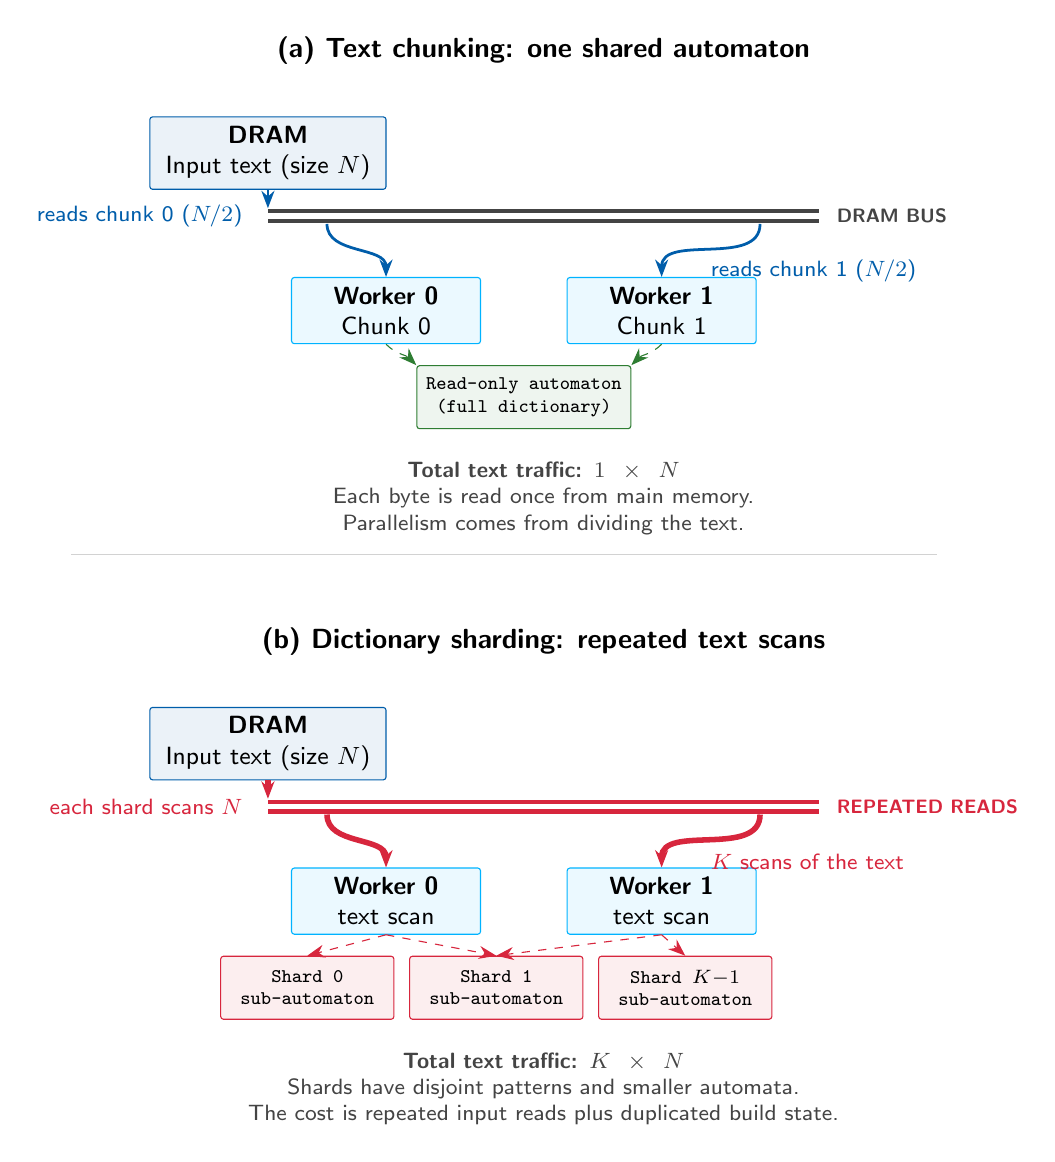
\begin{tikzpicture}[
    font=\small,
    >={Stealth[length=2.2mm]},
    title/.style={font=\bfseries},
    box/.style={draw=inkgray, rounded corners=1pt, minimum width=24mm, minimum height=8mm, align=center, fill=gray!6},
    dram/.style={box, draw=idpblue, fill=idpblue!8, minimum width=30mm},
    thread/.style={box, draw=idpcyan, fill=idpcyan!8},
    shard/.style={box, draw=inkgray, fill=gray!12, font=\scriptsize\ttfamily},
    note/.style={font=\footnotesize, text=inkgray, align=center},
    bus/.style={draw=inkgray, line width=1.5pt, double=white, double distance=2pt},
    arrow/.style={->, line width=1.0pt},
    heavyarrow/.style={->, line width=2.0pt, draw=warm},
]

    % =====================================================================
    % (a) PURE TEXT CHUNKING (1D)
    % =====================================================================
    \node[title] at (3.5, 3.8) {(a) Text chunking: one shared automaton};
    
    % DRAM input text
    \node[dram] (dram1) at (0, 2.5) {\textbf{DRAM}\\Input text (size $N$)};
    
    % Memory Bus
    \draw[bus] (0, 1.7) -- (7.0, 1.7);
    \node[anchor=west, font=\scriptsize\bfseries, text=inkgray] at (7.1, 1.7) {DRAM BUS};
    
    % Threads
    \node[thread] (t1_0) at (1.5, 0.5) {\textbf{Worker 0}\\Chunk 0};
    \node[thread] (t1_1) at (5.0, 0.5) {\textbf{Worker 1}\\Chunk 1};
    
    % Automaton
    \node[shard, fill=forestgreen!8, draw=forestgreen, minimum width=15mm] (auto1) at (3.25, -0.6) {Read-only automaton\\(full dictionary)};

    % Arrows from DRAM to threads (1x total transfer)
    \draw[arrow, idpblue] (dram1.south) to[out=-90, in=90] (0, 1.8);
    \draw[arrow, idpblue] (0.75, 1.6) to[out=-90, in=90] (t1_0.north);
    \draw[arrow, idpblue] (6.25, 1.6) to[out=-90, in=90] (t1_1.north);
    \node[note, anchor=east, text=idpblue] at (-0.2, 1.7) {reads chunk 0 ($N/2$)};
    \node[note, anchor=west, text=idpblue] at (5.5, 1.0) {reads chunk 1 ($N/2$)};

    % Connections to Automaton
    \draw[->, forestgreen, dashed] (t1_0.south) to[out=-45, in=135] (auto1.north west);
    \draw[->, forestgreen, dashed] (t1_1.south) to[out=-135, in=45] (auto1.north east);

    % Summary Note
    \node[note, anchor=north, text width=9.0cm] at (3.5, -1.3) {
        \textbf{Total text traffic: $1 \times N$}\\
        Each byte is read once from main memory.\\
        Parallelism comes from dividing the text.
    };

    % =====================================================================
    % (b) 2D COMPOSITION (Chunking + Sharding)
    % =====================================================================
    \begin{scope}[yshift=-7.5cm]
        \node[title] at (3.5, 3.8) {(b) Dictionary sharding: repeated text scans};
        
        % DRAM input text
        \node[dram] (dram2) at (0, 2.5) {\textbf{DRAM}\\Input text (size $N$)};
        
        % Memory Bus
        \draw[bus, draw=warm] (0, 1.7) -- (7.0, 1.7);
        \node[anchor=west, font=\scriptsize\bfseries, text=warm] at (7.1, 1.7) {REPEATED READS};
        
        % Threads & Shards
        \node[thread] (t2_0) at (1.5, 0.5) {\textbf{Worker 0}\\text scan};
        \node[thread] (t2_1) at (5.0, 0.5) {\textbf{Worker 1}\\text scan};
        
        % Sub-automata shards
        \node[shard, draw=warm, fill=warm!8, minimum width=22mm] (shard0) at (0.5, -0.6) {Shard 0\\sub-automaton};
        \node[shard, draw=warm, fill=warm!8, minimum width=22mm] (shard1) at (2.9, -0.6) {Shard 1\\sub-automaton};
        \node[shard, draw=warm, fill=warm!8, minimum width=22mm] (shard2) at (5.3, -0.6) {Shard $K{-}1$\\sub-automaton};

        % Multiplied text traffic (K shards = K reads per chunk)
        \draw[heavyarrow] (dram2.south) to[out=-90, in=90] (0, 1.8);
        
        % Thread 0 reads chunk 0 multiple times (once for each shard)
        \draw[heavyarrow] (0.75, 1.6) to[out=-90, in=90] (t2_0.north);
        \draw[heavyarrow] (6.25, 1.6) to[out=-90, in=90] (t2_1.north);
        
        \node[note, anchor=east, text=warm] at (-0.2, 1.7) {each shard scans $N$};
        \node[note, anchor=west, text=warm] at (5.5, 1.0) {$K$ scans of the text};

        % Connections to Shards
        \draw[->, warm, dashed] (t2_0.south) -- (shard0.north);
        \draw[->, warm, dashed] (t2_0.south) -- (shard1.north);
        \draw[->, warm, dashed] (t2_1.south) -- (shard1.north);
        \draw[->, warm, dashed] (t2_1.south) -- (shard2.north);

        % Summary Note
        \node[note, anchor=north, text width=9.0cm] at (3.5, -1.3) {
            \textbf{Total text traffic: $K \times N$}\\
            Shards have disjoint patterns and smaller automata.\\
            The cost is repeated input reads plus duplicated build state.
        };
    \end{scope}

    % Divider
    \draw[gray!35, line width=0.4pt] (-2.5, -2.6) -- (8.5, -2.6);

\end{tikzpicture}
\end{document}
